\documentclass[pdftex,12pt,xcolor=svgnames]{beamer}

\mode<presentation>
{
  \usetheme{boxes}
  \usecolortheme[named=MidnightBlue]{structure}
  %\setbeamercolor{normal text}{bg=NavajoWhite!20}
  %% \usefonttheme{serif}
  \setbeamertemplate{navigation symbols}{}
  % Show frame number and author name in footline
  \setbeamertemplate{frametitle}[default][center]
  \setbeamertemplate{footline}[frame number]
  \setbeamertemplate{items}[circle]
  %\addtobeamertemplate{footline}{\quad\textcolor{gray}{James Robert Lloyd}}{}
  % Set frame titles in small capitals
  %% \setbeamerfont{frametitle}{shape=\scshape,family=\rmfamily,size={\fontsize{16}{20}}}
  %% \setbeamercolor{frametitle}{bg=gray!60!white,fg=black}
  %% \setbeamercolor{frametitle}{bg=blue,fg=black}
  % Alerted text: blue (uncomment second line if theme sets alerted text to bold)
  \setbeamercolor{alerted text}{fg=blue}
  %\setbeamerfont*{alerted text}{}
  \setbeamertemplate{bibliography item}[text] %{\hbox{\donotcoloroutermaths$\blacktriangleright$}}
  \setbeamertemplate{bibliography entry title}{}
  \setbeamertemplate{bibliography entry author}{}
  \setbeamertemplate{bibliography entry note}{}
  \setbeamertemplate{bibliography entry location}{}

}
\usepackage[english]{babel}
\usepackage[latin1]{inputenc}
\usepackage{times}
\usepackage[T1]{fontenc}
\usepackage{hyperref}
\usepackage{multimedia}
\usepackage{eepic}
\usepackage{graphicx}
%\usepackage[nohug]{latexinclude/diagrams}
\usepackage{tikz}
\usetikzlibrary{calc}

%% \newcommand{\footlineextra}[1]{
%%     \begin{tikzpicture}[remember picture,overlay]
%%         \node[yshift=1.5ex,anchor=south east] at (current page.south east)
%% {#1};
%%     \end{tikzpicture}
%% }

\newcommand{\footlineextra}[1]{
    \begin{tikzpicture}[remember picture,overlay]
        \node[xshift=-5ex,yshift=-0.5ex,anchor=south east] at (current page.south east)
             {\mbox{\tiny \textcolor{MidnightBlue}{#1}}};
    \end{tikzpicture}
}

\def\sectionframe#1{
  {
    \setbeamertemplate{footline}{\empty}
    \begin{frame}{}
      \begin{center}
        \huge\sc #1
      \end{center}
    \end{frame}
  }
}


\usepackage{etex}

\usepackage{tabularx}
\usepackage{include/picins}
\usepackage{include/preamble}
\usepackage{setspace}
\usepackage{xcolor}
\usepackage{tikz}
\usepackage{listings}

\usetikzlibrary{shapes.geometric,arrows,chains,matrix,positioning,scopes,calc,shapes.arrows}

%\usepackage{algorithm}
%\usepackage{algpseudocode}

% Python code definition

\definecolor{Blue}{rgb}{0.0,0.0,1.0}
\lstloadlanguages{Python}%
\lstset{language=Python,
        frame=none,
        basicstyle=\tiny\ttfamily\bfseries,
        keywordstyle=[1]\color{Blue},
        keywordstyle=[2]\color{Purple},
        commentstyle=\usefont{T1}{pcr}{m}{sl}\color{Green},
        keepspaces=true,
        }

\lstset{language=Python} 
\lstset{columns=fullflexible}

%%%%%%%%%%%%%%%%%%%%%%%%%%%%%%%%%%%%%%%%%%%
%
% Some look and feel definitions
%
%%%%%%%%%%%%%%%%%%%%%%%%%%%%%%%%%%%%%%%%%%%

\setlength{\columnsep}{0.03\textwidth}
\setlength{\columnseprule}{0.0018\textwidth}
\setlength{\parindent}{0.0cm}
  
\tikzstyle{mybox} = [draw=white, rectangle]
\tikzset{hide on/.code={\only<#1>{\color{white}}}}

\definecolor{camlightblue}{rgb}{0.601 , 0.8, 1}
\definecolor{camdarkblue}{rgb}{0, 0.203, 0.402}
\definecolor{camred}{rgb}{1, 0.203, 0}
\definecolor{camyellow}{rgb}{1, 0.8, 0}
\definecolor{lightblue}{rgb}{0, 0, 0.80}
\definecolor{white}{rgb}{1, 1, 1}
\definecolor{whiteblue}{rgb}{0.80, 0.80, 1}

\newcolumntype{x}[1]{>{\centering\arraybackslash\hspace{0pt}}m{#1}}
\newcommand{\tabbox}[1]{#1}

\hypersetup{colorlinks=true,citecolor=blue}

\newcommand{\primal}{elementary}
\newcommand{\Primal}{Elementary}
\newcommand{\numhypers}{N}
\newcommand{\hypers}{{\boldsymbol{\theta}}}
\newcommand{\params}{\vw}
\newcommand{\numsteps}{T}
\newcommand{\decay}{\gamma}
\newcommand{\decays}{{\boldsymbol{\decay}}}
\newcommand{\stepsize}{\alpha}
\newcommand{\stepsizes}{{\boldsymbol{\stepsize}}}
\newcommand{\gradparams}{\nabla_\params L(\params_t, \hypers, t)}

%%%%%%%%%%%%%%%%%%%%%%%%%%%%%%%%%%%%%%%%%%%
%
% The talk
%
%%%%%%%%%%%%%%%%%%%%%%%%%%%%%%%%%%%%%%%%%%%

\title{Why not use gradients?}

\author{
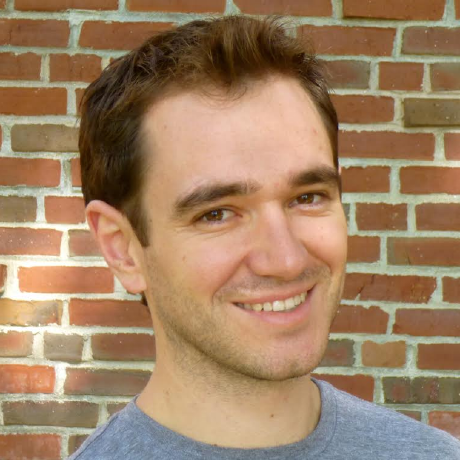
\includegraphics[height=0.16\textwidth]{talkfigs/dougal}
\qquad
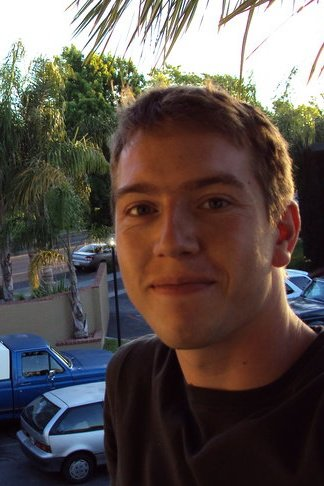
\includegraphics[height=0.16\textwidth, trim=20mm 25mm 0mm 25mm, clip]{talkfigs/david2}
\qquad
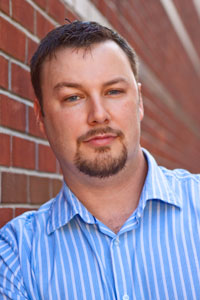
\includegraphics[height=0.16\textwidth]{talkfigs/adams}
\\
Dougal Maclaurin, David Duvenaud, Ryan Prescott Adams}

\institute{Harvard University}

\begin{document}

\frame[plain] {\titlepage}



\frame[plain]{
\frametitle{Motivation} DM
\begin{itemize} 
\item Hyperparameter optimization is important
\item Can't scale to high dimensions because we don't have gradients
\item Only one number per evaluation.
\item How do we normally do things?
\end{itemize}}

\frame[plain]{\frametitle{Reverse-mode Differentiation} DM}

\frame[plain]{\frametitle{FunkyYak: Automatic Differentiation} 
\url{github.com/HIPS/FunkyYak}}

\frame[plain]{\frametitle{FunkyYak Simple Example}
\begin{columns}
\begin{column}{5.5cm}
\lstinputlisting{code/sinusoid.py} 
\end{column}
\begin{column}{5cm}
	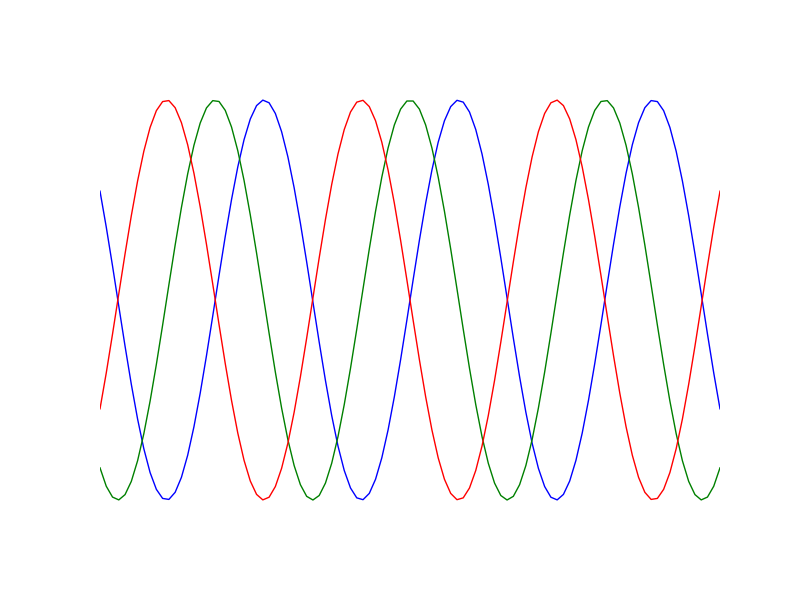
\includegraphics[width=6cm]{code/sinusoid.png}
\end{column}
\end{columns}}

\frame[plain]{\frametitle{FunkyYak Complicated Example}
\begin{columns}
\begin{column}{5.5cm}
\lstinputlisting{code/sinusoid-taylor.py} 
\end{column}
\begin{column}{5cm}
	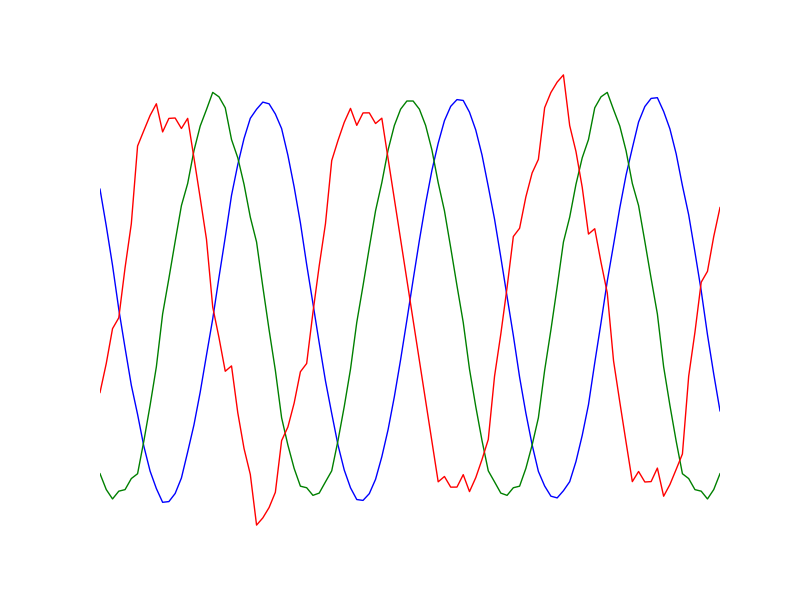
\includegraphics[width=6cm]{code/sinusoid_taylor.png}
\end{column}
\end{columns}}

\frame[plain]{\frametitle{FunkyYak Higher Derivatives}
\begin{columns}
\begin{column}{5.5cm}
\lstinputlisting{code/tanh.py}
\end{column}
\begin{column}{5cm}
	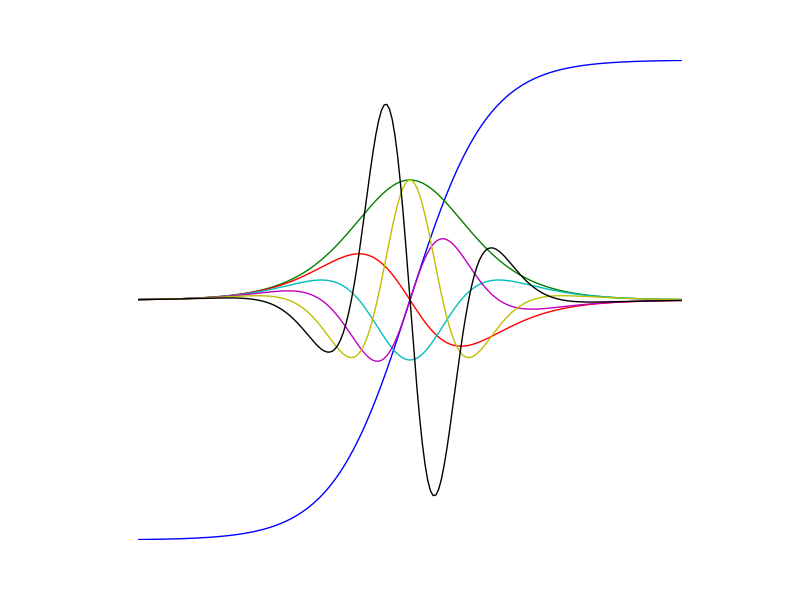
\includegraphics[width=6cm]{code/tanh.png}
\end{column}
\end{columns}}

\frame[plain]{\frametitle{SGD is just a function}
\includegraphics<1>[width=0.9\columnwidth]{talkfigs/learning_curves_1.pdf}%
\includegraphics<2>[width=0.9\columnwidth]{talkfigs/learning_curves_2.pdf}%
\includegraphics<3>[width=0.9\columnwidth]{talkfigs/learning_curves_3.pdf}%
}

\frame[plain]{\frametitle{Example uses of hyper-gradients: learning rates}
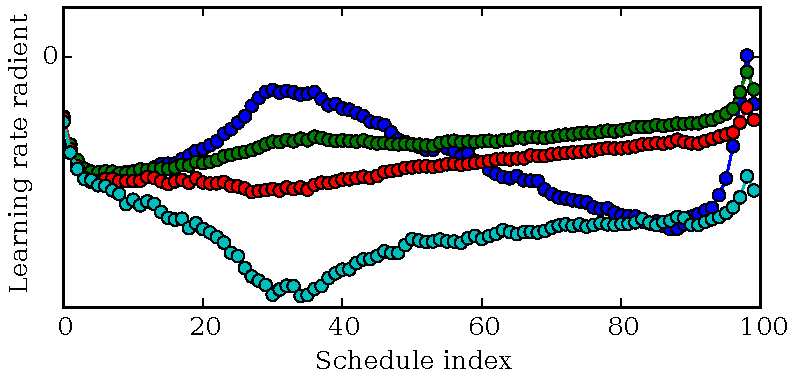
\includegraphics[width=\columnwidth]{../experiments/Feb_3_training_schedules/5_initial_gradient/schedules_small.pdf}}

\frame[plain]{\frametitle{Example uses of hyper-gradients: learning rates}
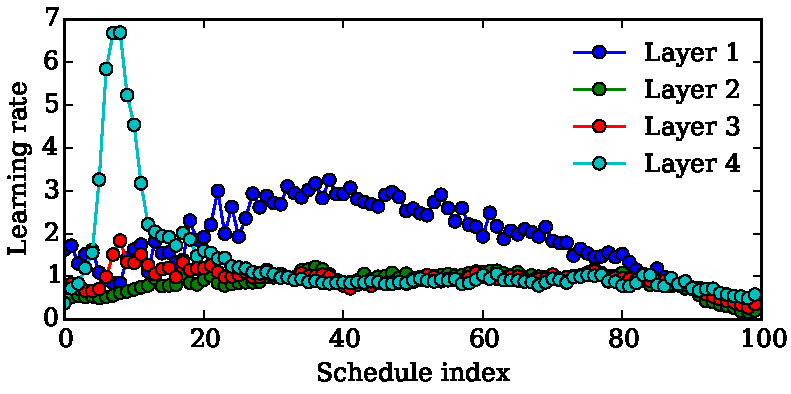
\includegraphics[width=\columnwidth]{../experiments/Feb_3_training_schedules/3_adam_50/schedules_small.pdf}
}

\frame[plain]{\frametitle{Optimizing initialization distributions} 
\begin{center}
\begin{tabular}{cc}
 Biases & Weights \\
\hspace{-1em}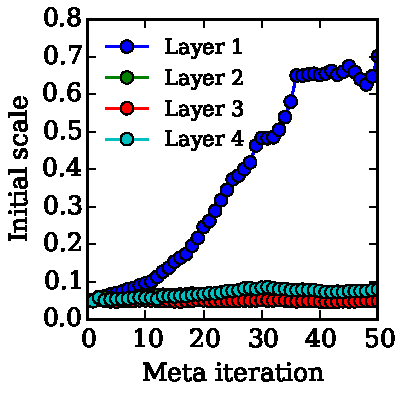
\includegraphics[width=0.5\columnwidth, height=0.5\columnwidth]{../experiments/Feb_3_training_schedules/3_adam_50/init_bias_learning_curve.pdf} &
\hspace{-1em}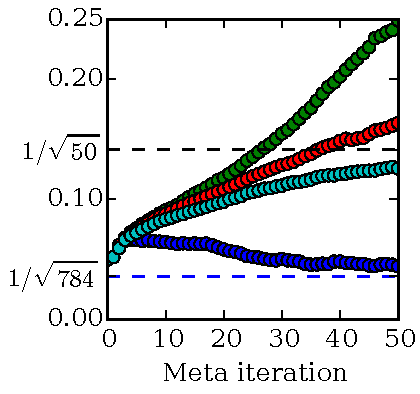
\includegraphics[width=0.5\columnwidth, height=0.5\columnwidth]{../experiments/Feb_3_training_schedules/3_adam_50/init_weight_learning_curve.pdf}
\end{tabular}
\end{center}
}

\frame[plain]{\frametitle{Optimizing training data} 
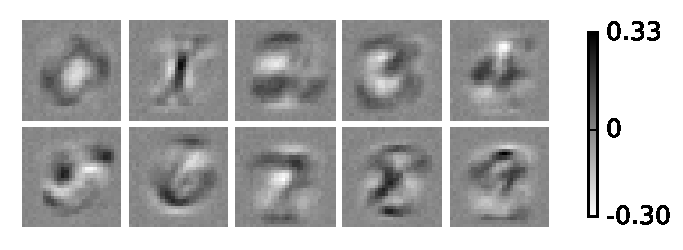
\includegraphics[width=\columnwidth]{../experiments/Jan_19_optimize_data/9_color_bar/fake_data.pdf}} 

\frame[plain]{\frametitle{Optimizing architecture/regularization} DD}

\frame[plain]{\frametitle{Optimizing regularization: polyglot}
\begin{center}
\begin{tabular}{cc}
\hspace{-3mm}\rotatebox{90}{\qquad Rotated \qquad \quad Original} & 
\hspace{-3mm}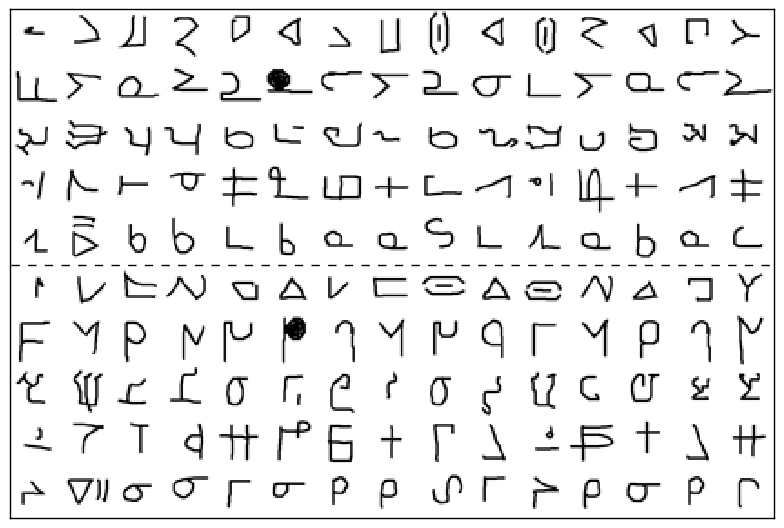
\includegraphics[width=0.85\columnwidth]{../experiments/Feb_4_augmented_omniglot/2_rotated_90/all_alphabets.png}
\end{tabular}
\end{center}
}

\newcommand{\omniimagea}[2]{\parbox{4em}{\includegraphics[width=1.4cm]{../experiments/Feb_4_augmented_omniglot/2_rotated_90/minifigs/learned_corr_#1_#2.pdf}}}%
\newcommand{\omniimageb}[1]{\omniimagea{#1}{0} & \omniimagea{#1}{1} & \omniimagea{#1}{2}}%

\frame[plain]{\frametitle{Optimizing regularization: polyglot}
\begin{center}
\begin{tabular}{c@{\hskip 0.9em}ccc@{\hskip 0.9em}c@{\hskip 0.9em}c}%
\renewcommand{\tabcolsep}{1pt}
& Input   & Middle  & Output & Train & Test\\
& weights & weights & weights & error & error \\
\parbox{3.7em}{Separate networks} & \omniimageb{no_sharing}      & 0.61 & 1.34\\ \hline
\parbox{3.7em}{Tied weights}      & \omniimageb{full_sharing}    & 0.90 & 1.25\\ \hline
\parbox{3.7em}{Learned sharing}   & \omniimageb{learned_sharing} & 0.60 & \bf 1.13
\end{tabular}
\end{center}
}

\frame[plain]{\frametitle{Limitations: Chaotic learning dynamics}
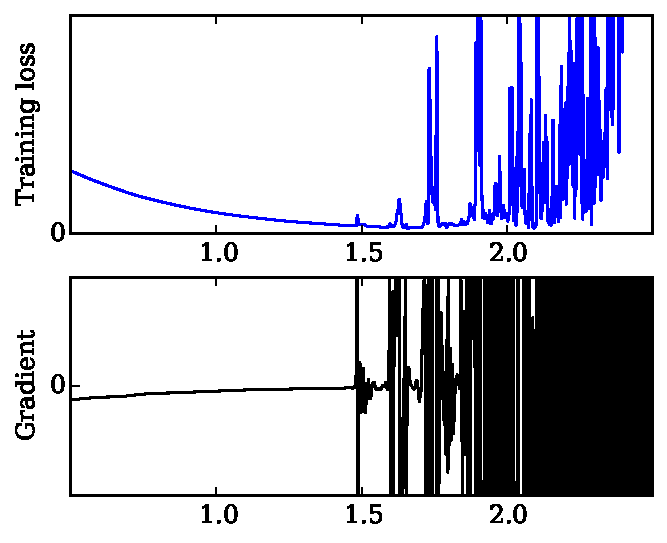
\includegraphics[width=0.9\columnwidth]{../experiments/Jan_14_learning_rate_wiggliness/3/chaos.pdf}}

\frame[plain]{\frametitle{Other possible applications} DM}

\frame[plain]{\frametitle{Why hasn't this been done before?} % DM
Domke did it for small problems}

\frame[plain]{\frametitle{Memory is the limiting factor} %DM
\begin{itemize}
\item Memory required is $N \times T$.
\item Don't need random access.
\item Could eliminate memory burden if we could recalculate intermediate parameters values as we go backwards through the learning process.
\end{itemize}}

\frame[plain]{\frametitle{Can't reverse naively}
\includegraphics<1>[width=0.9\columnwidth]{../experiments/Jan_25_Figure_1/4_naive_reverse/learning_curve_forward.pdf}
\includegraphics<2>[width=0.9\columnwidth]{../experiments/Jan_25_Figure_1/4_naive_reverse/learning_curve_reverse.pdf}
}

\frame[plain]{\frametitle{Entropy and Optimization}  %DM
[TODO: Figure of dividing by 2

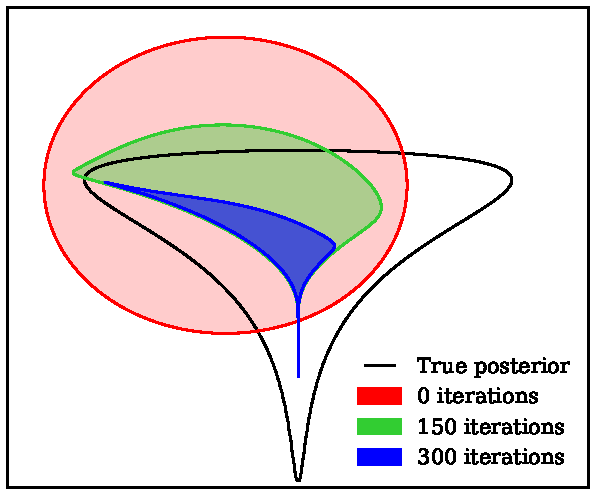
\includegraphics[width=0.9\columnwidth]{talkfigs/dists}
}

\frame[plain]{\frametitle{Storing the extra bits on a tape} %DM
\begin{itemize} 
\item Simple algorithm that only uses arithmetic operations
\item Could be any LIFO coding method.
\end{itemize}
}

\frame[plain]{\frametitle{Summary}  %DM
\begin{itemize}
\item Learning algorithms can be differentiated like any other.
\item This lets us do meta-learning.  Many applications besides deep learning: reinforcement learning.
\item Deep connection between learning and entropy.
\end{itemize}
}



\end{document}
